\chapter{Credit Scoring}

\section{Introduction}
Credit scoring is a method used by financial institution globally to assess whether a customer should be taken on. This can be for a variety of services such as credit cards, loans, mortgages, etc. It's development originated from the need of risk vs rewards. Lenders needed a way of determining if a potential customer would be able to pay back their credit and as such not costing the lender money by taking on creditees which end up being unable to repay the debt. A credit score is usually just a number indicating your quality as a creditee. The scale of the score can vary on which lender is providing the score but usual ones are 0-999 or 0-500 with the lower the score the less likely you would be offered the service. \\

Although used globally, there is no widely accepted "perfect" model or method. All companies assess their customers differently, a customer could be rejected from one lender and be accepted by another based on what they would define as an acceptable client. Even within companies the models and methods can change due to new circumstances and the changing financial climet. What previously could of been a strong predictor of a bad client could now be insignifcant. A recent example of this is the technology development of mobile phones. Previously, if a client did not have access home phone this could be an indicator of a possible bad client. Now, with the development and wide public access to mobile phones, access to a home phone has become mostly irrelevant with most of the public having no use for them anymore. Changes such as this and others require lenders to be constantly evaluating how they assess customers to prevent the rejection of good clients and the accepting of bad ones.

\section{Modelling}
Credit score modelling is often discrete based with the most common being a logistic regression with the response variable being either a good $(y=0)$ or bad customer $(y=1)$. Predictors can be a variety of variable such as personal characteristics, age, gender or economic status e.g. car owner, home owner/rentor etc, to financial characteristics like amont of current debt and repayment statuses. One thing to note, certain personal characteristics are off limit to company due to discrimination laws. Predictors such as race, may be shown to have some use in scoring but cannot be used as the model would become discriminatory.

\section{WOE and IV}
Weight of evidence (WOE) is a popular method used in score card modelling, often used because the variables used in credit scoring can have a large amount of categories which cause impractiallities when converting these to dummy variables. WOE is an alternative to that, rather than create a large amount of dummy variables, the method produces a numerical value (weight of evidence) for each category which is prdouced by (\ref{WOE}). with $f()$ being the distribution of category $X$ for goods and bads. These value then replace their respective categorical value when modelling the scorecard.

\begin{equation}\label{WOE}
WOE = \ln \frac{f(X=x|y=0)}{f(X=x|y=1)}
\end{equation}

IV, the information value. Is a measure of the weight of evidence for categories $IV \geq 0$. A value of 0 indicates the variable has no predictive power i.e. no valueable information in the variable. IV is calculated by (\ref{IV}). A guideline produced by Bailey\cite{bailey2004credit} is below for evaluating the IV values.

\begin{equation}\label{IV}
\textup{IV} = \sum (\% \textup{ of Bad} - \% \textup{ of Good}) \cdot \textup{WOE}
\end{equation}

\begin{figure}[H]
	\centering
	\begin{tabular}{l l l l}
	IV	&Recommendation \\
	\hline
	Less than 0.03			&Poor Predictor \\
	From 0.03 to less than 0.10	&Weak Predictor \\
	From 0.10 to less than 0.30	&Average Predictor \\
	From 0.30 to less than 0.50	&Strong Predictor \\
	Over 0.50				&Very Strong Predictor \\
	\end{tabular}
	\caption{Information Value Table \label{IV}}\cite{bailey2004credit}
\end{figure}

\section{Performance Evaulation}

\subsection{ROC and AUC}
ROC, Receiver Operating Characteristic. Was a method of analysis developed during World War II under "Signal Detection Theory". It was originally used for radar operators and their ability to determine if a blip on screen was an enemy or just noise, hence the name Receiver Operating Characteristics.\cite{tape2000using} Since then, the method has been applied into a variety of fields for visuallising the accuary of classification models. \\

Understanding the ROC Curve is relatively simple, the plot is the false positive rate against true positive rate for different cutoff points. The true positive rate is seen as the sensitivity and the false positive being (1 - specificity) An example figure can be found below, the higher the curve, the more accurate the model can be seen as, with the neutral line going 45 degrees through the plot can be seen as the model being the same as a 50/50 guess on the outcome. In some cases these curves can overlap and cause some ambiguity on which curve is overall the best so the measure used to remove this amiguity is the AUC, Area under the curve (\ref{AUC}). A higher AUC inidicates a stronger disciminatory power with 0.5 being none and 1 being a "perfect model". As such the model with a higher AUC can be considered "a better model". Generally, an $AUC > 0.8$ is considerd good.

\begin{equation}\label{AUC}
A = \int_{c}^{} F_1(c){F_0}'(c) dc
\end{equation}

A more common representation of the AUC is the gini coefficient (\ref{GINI}). A linear transformation of the AUC to allow the measure to have a preferred 0 to 1 scale rather than 0.5 to 1.

\begin{equation}\label{GINI}
gini = (2 \cdot AUC) - 1
\end{equation}

\begin{figure}[!ht]
	\centering
	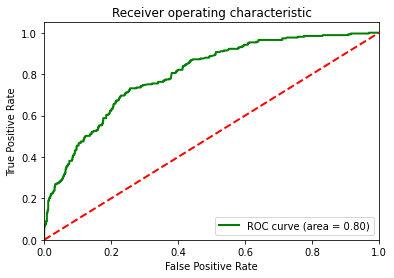
\includegraphics[scale=1.00]{figs/roc_example.png}
	\caption{ROC Example \label{roc_example}}
\end{figure}

\subsection{K-S Statistic}

The K-S Statistic (Kolmogorov-Smirnov Statistic) is a measurement of the scorecards ability to seperate the goods from bads. The K-S Statistic is the maximum distance between the cumulative distributions of both the goods and bads, or alterntively, if $F_{g}(x)$ is the cumulative distribution of goods and bads is $F_{b}(x)$ where $x$ is the score then the KS Statistic is (\ref{KS})

\begin{equation}\label{KS}
KS = max(F_{g}(x) - F_{b}(x))
\end{equation}

The statistic can be expressed visually by plotting the cumlative distributions as seen below. An issue of this measurement is that it only provides the score at which the scordcard seperates the goods and bads the most. The cutoff score for the card might not necessarily be this score and a higher K-S score does not imply the scorecard is a better fit. 

\subsection{Divergence}

Divergence is a measurement of the distributions of goods and bads. The idea is that the scorecard on average will assign a lower score to bads than goods i.e. $\mu_{b} < \mu_{g}$. Divergence is a way to assess this performance. 

\section{Cut-off}
A scorecard in simple terms is just a method producing a score for each individual. To put the scorecard into use the difference between the scores needs to be classified this is done by a cut-off score. This score is a point on the scorecard which would seperate accepted applicants from rejected. A simple cut-off method would be to have a single score, any applicants above the score are accepted and anyone below the score is rejected. The benefit of a simple method is the ability to quickly process applicants and move desired applicants onto the next stage faster. The issue with the single cutoff comes with the applicants that are close to the cutoff, having a strict cut-off can cause a company to take on bad applicants or reject good applicants where futher investigation would prove the applicant more likely to be the opposite. \\

An alternative to this would be a two score cut-off. This would be done by having two scores like $ \textup{Rejected } < S_{1} < \textup{ Refer } < S_{2} < \textup{ Accepted}$. Any score above $S_{2}$ is automatically accepted and any below $S_{1}$ is rejected. Scores which the land in between and moved to a referral stage where a lender can further look into the applicants case by case to decide the outcome. This comes with added benefit of removing the issue of applicants close to the single cutoff. The idea is that with the lenders insight, more good applicants will be accepted and more bads rejected compared to the single cutoff, thus possibly reducing the bad rate of accepted applicants. \\

The cut-off scores can be determined by varying factors which can change depending on the companies interest. Four of these are specified by Bailey \cite{bailey2004credit}. Acceptance rate, the percentage of all applicants accepted by the cut-off. Overall bad rate, the percentage of all accepted applicants that end up being bads. Marginal bad rate, the percentage of accepted applicancts that are bad close to the cut-off score. Profitability, the possible profit from goods minus the loss from bads. Depending on the situation of the business and its goals would determine the importance of each factor with overal bad rate being the usual priority.

\section{Population Stability Index}



%\begin{figure}[H]
%	\centering
%	\includegraphics[scale=0.50]{figs/White_Pop}
%	\caption{\% Of White Alone population in Boston Metropolitan \label{W_Pop}}\cite{DataCommon}
%\end{figure}
%
%\begin{figure}[H]
%	\centering
%	\includegraphics[scale=0.50]{figs/Black_Pop}
%	\caption{\% Of Black or African American population in Boston Metropolitan \label{B_Pop}}\cite{DataCommon}
%\end{figure}
%
%\begin{figure}[H]
%	\centering
%	\includegraphics[scale=0.50]{figs/Asian_Pop}
%	\caption{\% Of Asian alone population in Boston Metropolitan \label{A_Pop}}\cite{DataCommon}
%\end{figure}

%The state of Metro Boston's Economy is considered one of the stronger economies when compared to state, national averages and globally. In a report done by Brookings Insitute  in 2014 of 300 of the world's largest metropolitan economies, Boston ranked in at 24th in the world for GDP with \$ 360,110 million and 4th for GDP per capita with \$ 76,204.\cite{GMM} The economy of Boston is heavily influenced by its' financial, business and technological services along with the city having strong educational and medical sectors. Home to leading medical schools Tufts University and Harvard University and also Massachusetts Institute of Technology, International students come from come from all over the world to study at the world class universities in Boston. The affect of having prestigious universities in a city can have a large impact on the economy of the city. The high skilled work force they produce has attracted the knowledge-based industries on which Boston's economy is now heavily based. Examples of these are the high technology, biotechnology and financial service. Boston boasts a very strong educational sector and produces numerous skilled professionals. Along with these, Boston is also a popular tourist destination with both domestic and international visitors. In 2014 visitors spent \$12.2 billion.\\
%
%The costs of living in Boston according to Numbeo's index can be considered to be at a high standard.\cite{NUM} The index can be seen as the cost of living in an area relative to what it is in New York. In 2014 Boston was ranked 121 of 473 globally and 14 of 94 in North America with a cost of living index of 92.94 (New York being 100.00). \\
%
% The city's median household income is one of the higher for the Nations cities with average value of \$58,263. Although the city still contains the racial disparities for incomes seen across the country. The median household income is comparatively very low when you reach the inner part of the city with some areas having an average income less than \$ 40,000. This also follows along with the racial income gaps, with the average median income for an African American household being at \$40,128 and \$80,515 for a White household.\cite{CityData}
 
%\begin{figure}[H]
%	\centering
%	\includegraphics[scale=0.50]{figs/Med_Inc}
%	\caption{Median household income \label{Med_Inc}}\cite{DataCommon}
%\end{figure} 
%
%\begin{figure}[H]
%	\centering
%	\begin{tabular}{l l l l}
%	Date	&US		&Massachusets	&Boston \\
%	\hline
%	2015	&\$55,775	&\$70,628	&\$78,800 \\
%	2014	&\$53,719	&\$69,240	&\$75,754 \\
%	2013	&\$53,167	&\$67,939	&\$74,186 \\
%	2012	&\$53,031	&\$67,451	&\$74,057 \\
%	2011	&\$53,223	&\$66,246	&\$73,197 \\
%	2010	&\$54,405	&\$67,479	&\$73,945 \\
%	2009	&\$55,478	&\$70,789	&\$76,592 \\
%	2008	&\$57,276	&\$71,997	&\$78,558 \\
%	2007	&\$58,003	&\$71,291	&\$77,895 \\
%	2006	&\$56,957	&\$70,490	&\$75,405 \\
%	2005	&\$56,122	&\$69,402	&\$75,329 \\
%	\end{tabular}
%	\caption{Historical Inflation Adjusted Median Household Income for Boston \label{Table1}}\cite{HouseholdIncome}
%\end{figure}